\section{Focal lenght of paraffin wax lens} \label{sec:FocalLenght}

To further investigate microwaves, it is necessary to produce collimated rays. For that a paraffin wax lens was used which focal point has to be determined.
This was archieved by placing a wax lens between transmitter and receiver. The distance between the transmitter and the las is $g = (80 \pm 1)cm$. The 
receiver is placed with maximal possible distance to the lense and then progressively moved towards it. The radiation was measured in every step.
To determine the peak radiation level, a smooth curve was fitted to the experimental data and it's maximum was determined to $b' = (151.8 \pm 6.0)cm$. 
The plot is shown in fig. \ref{fig:brennweite}.\\
The focal length was then calculated using the thin-lense equation:
\begin{equation}
    f = \frac{g \cdot b}{g + b} \quad \text{with} \quad b = b' - g
\end{equation}
which results in a focal lenght of $(f = 37.84 \pm 0.48(cm)$. In the following parts of the experiment, the focal lenght was roughly placed at 40 cm, such that
the rays would be collimated.

\begin{figure}
\centering
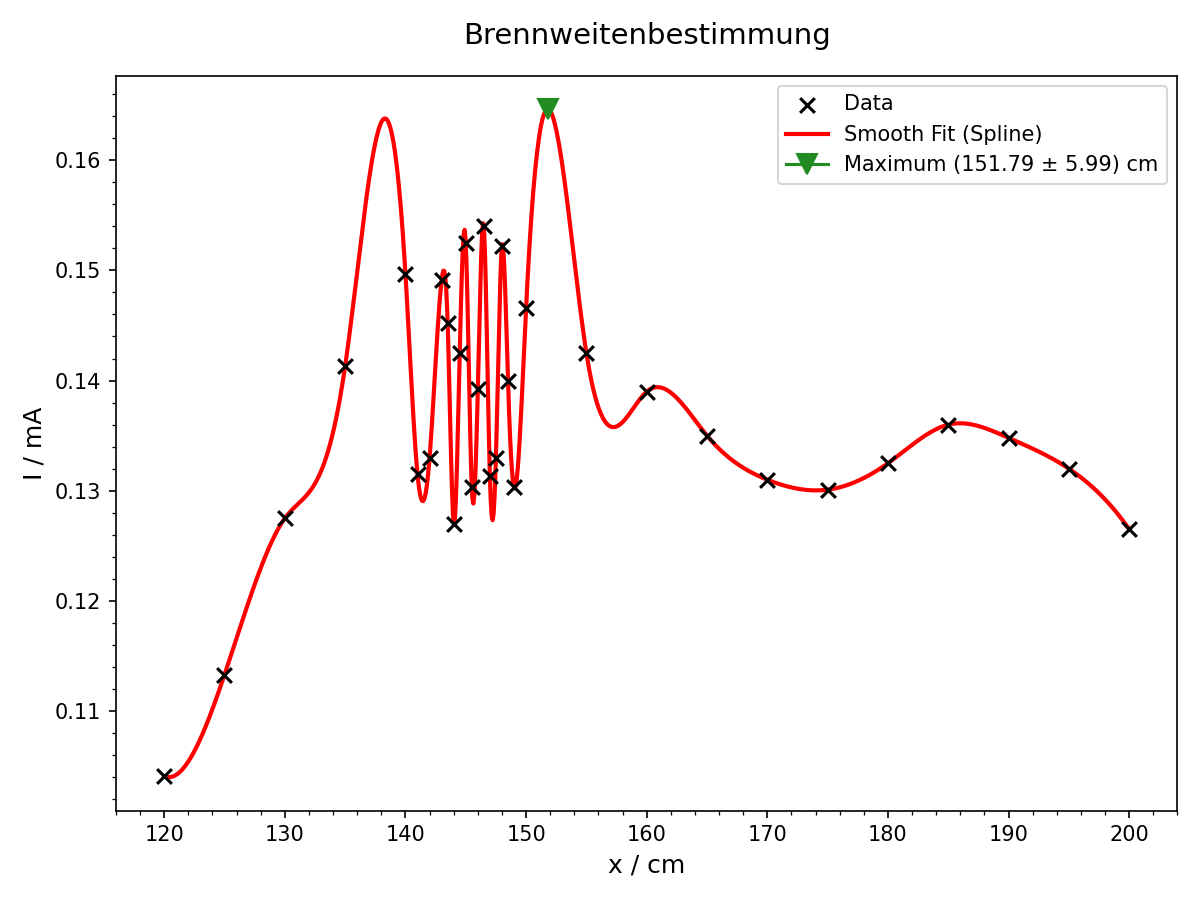
\includegraphics[width=0.5\textwidth]{../Images/brennweite_fit_clean.png}
\caption{Intensity profile of the microwave radiation in relation to it's distance from the lens.}
\label{fig:brennweite}
\end{figure}